\textbf{Testumgebung}

Die Messungen wurden mit einem Notebook aufgenommen, welches
folgende Hardwarekonfigurationen besitzt.

\textit{
	LENOVO Thinkpad t410 Modell 2522-w29 \newline
	\textbf{Prozessor}: Intel Core i5 520M (2 Kerne mit Hyperthreading $\stackrel{\wedge}=$ 4 Threads)\\
	\textbf{Arbeitsspeicher}: 4 GB DDR3	
	}

Da eine ähnliche Hardware bei einer Verwendung des Protokolls auf dem Mars
weniger zu erwarten ist, sind die Größenordnungen der nachfolgenden Ergebnisse
nur ein Richtwert. Für die folgenden Betrachtungen sind die Beziehungen und
Entwicklungen der einzelnen Werte zueinander wichtig, welche mit schwächerer
Hardware nahezu identisch sind. Zum Vergleich der Hardware des weniger
performanten Rovers \textit{Curiosity} sei auf das Kapitel
\ref{cap:standDerTechnik} verwiesen.
\\

\textbf{Ergebnisse und Diskussion}

Alle nachfolgend aufgeführten Diagramme und Messwerte sind noch einmal im Anhang
in einer größeren Darstellung aufgeführt.\newline
Das Protokoll wird grundlegend mit zwei verschiedenen Kompilereinstellungen
getestet. Dies sind die Geschwindigkeits- (\glqq O$2$ \grqq) und die
Quellcodegrößenoptimierung (\glqq Os \grqq).
\newline
% Hypothese 1
Bei O$2$ sollte die Laufzeit stets kleiner sein als bei Os. Weiterhin ist
anzunehmen, dass der Zeitbedarf bei größerwerdenden Datenpaketen kontinuierlich
ansteigt.
\newline
% Methodik 1
Dabei wurde untersucht, wie lange das Protokoll für die Verarbeitung von Texten
verschiedener Größe benötigt, die keine relevanten Bereiche besitzen. Dafür
wurden Dateien mit verschiedenen Größen von $2$ Bytes bis $10$ Millionen Byte 
angelegt, durch das Programm eingelesen und der Schnittstelle des Protokolls
übergeben. Vor der Übergabe der Daten wurde das Modul gelöscht und neu erstellt.
Dadurch ist ein Messen der reinen Verarbeitungsdauer gewährleistet. Für einen
aussagekräftigeren Wert und um potentielle Messungenauigkeiten zu kompensieren,
werden die Messungen für jede Einstellung $10$ Mal wiederholt und der Mittelwert
gebildet.
% Auswertung 1
\newline
Die Abbildung \ref{fig:diagrammInitial_worp} zeigt grafisch die Ergebnisse der
Messreihen. Dabei ist die
Laufzeit in $\mu s$ über die Textgröße in Byte logarithmisch aufgetragen.
Entgegen den Erwartungen hat die Geschwindkeitsoptimierung für relativ
kleine Textgrößen noch keinen großen Einfluss. Erst ab einer Größe von
$5.000.000$ Byte ($99\ \mu s$) ist ein Geschwindigkeitsprofit zu
verzeichnen.

\begin{figure}[H]
	\centering
	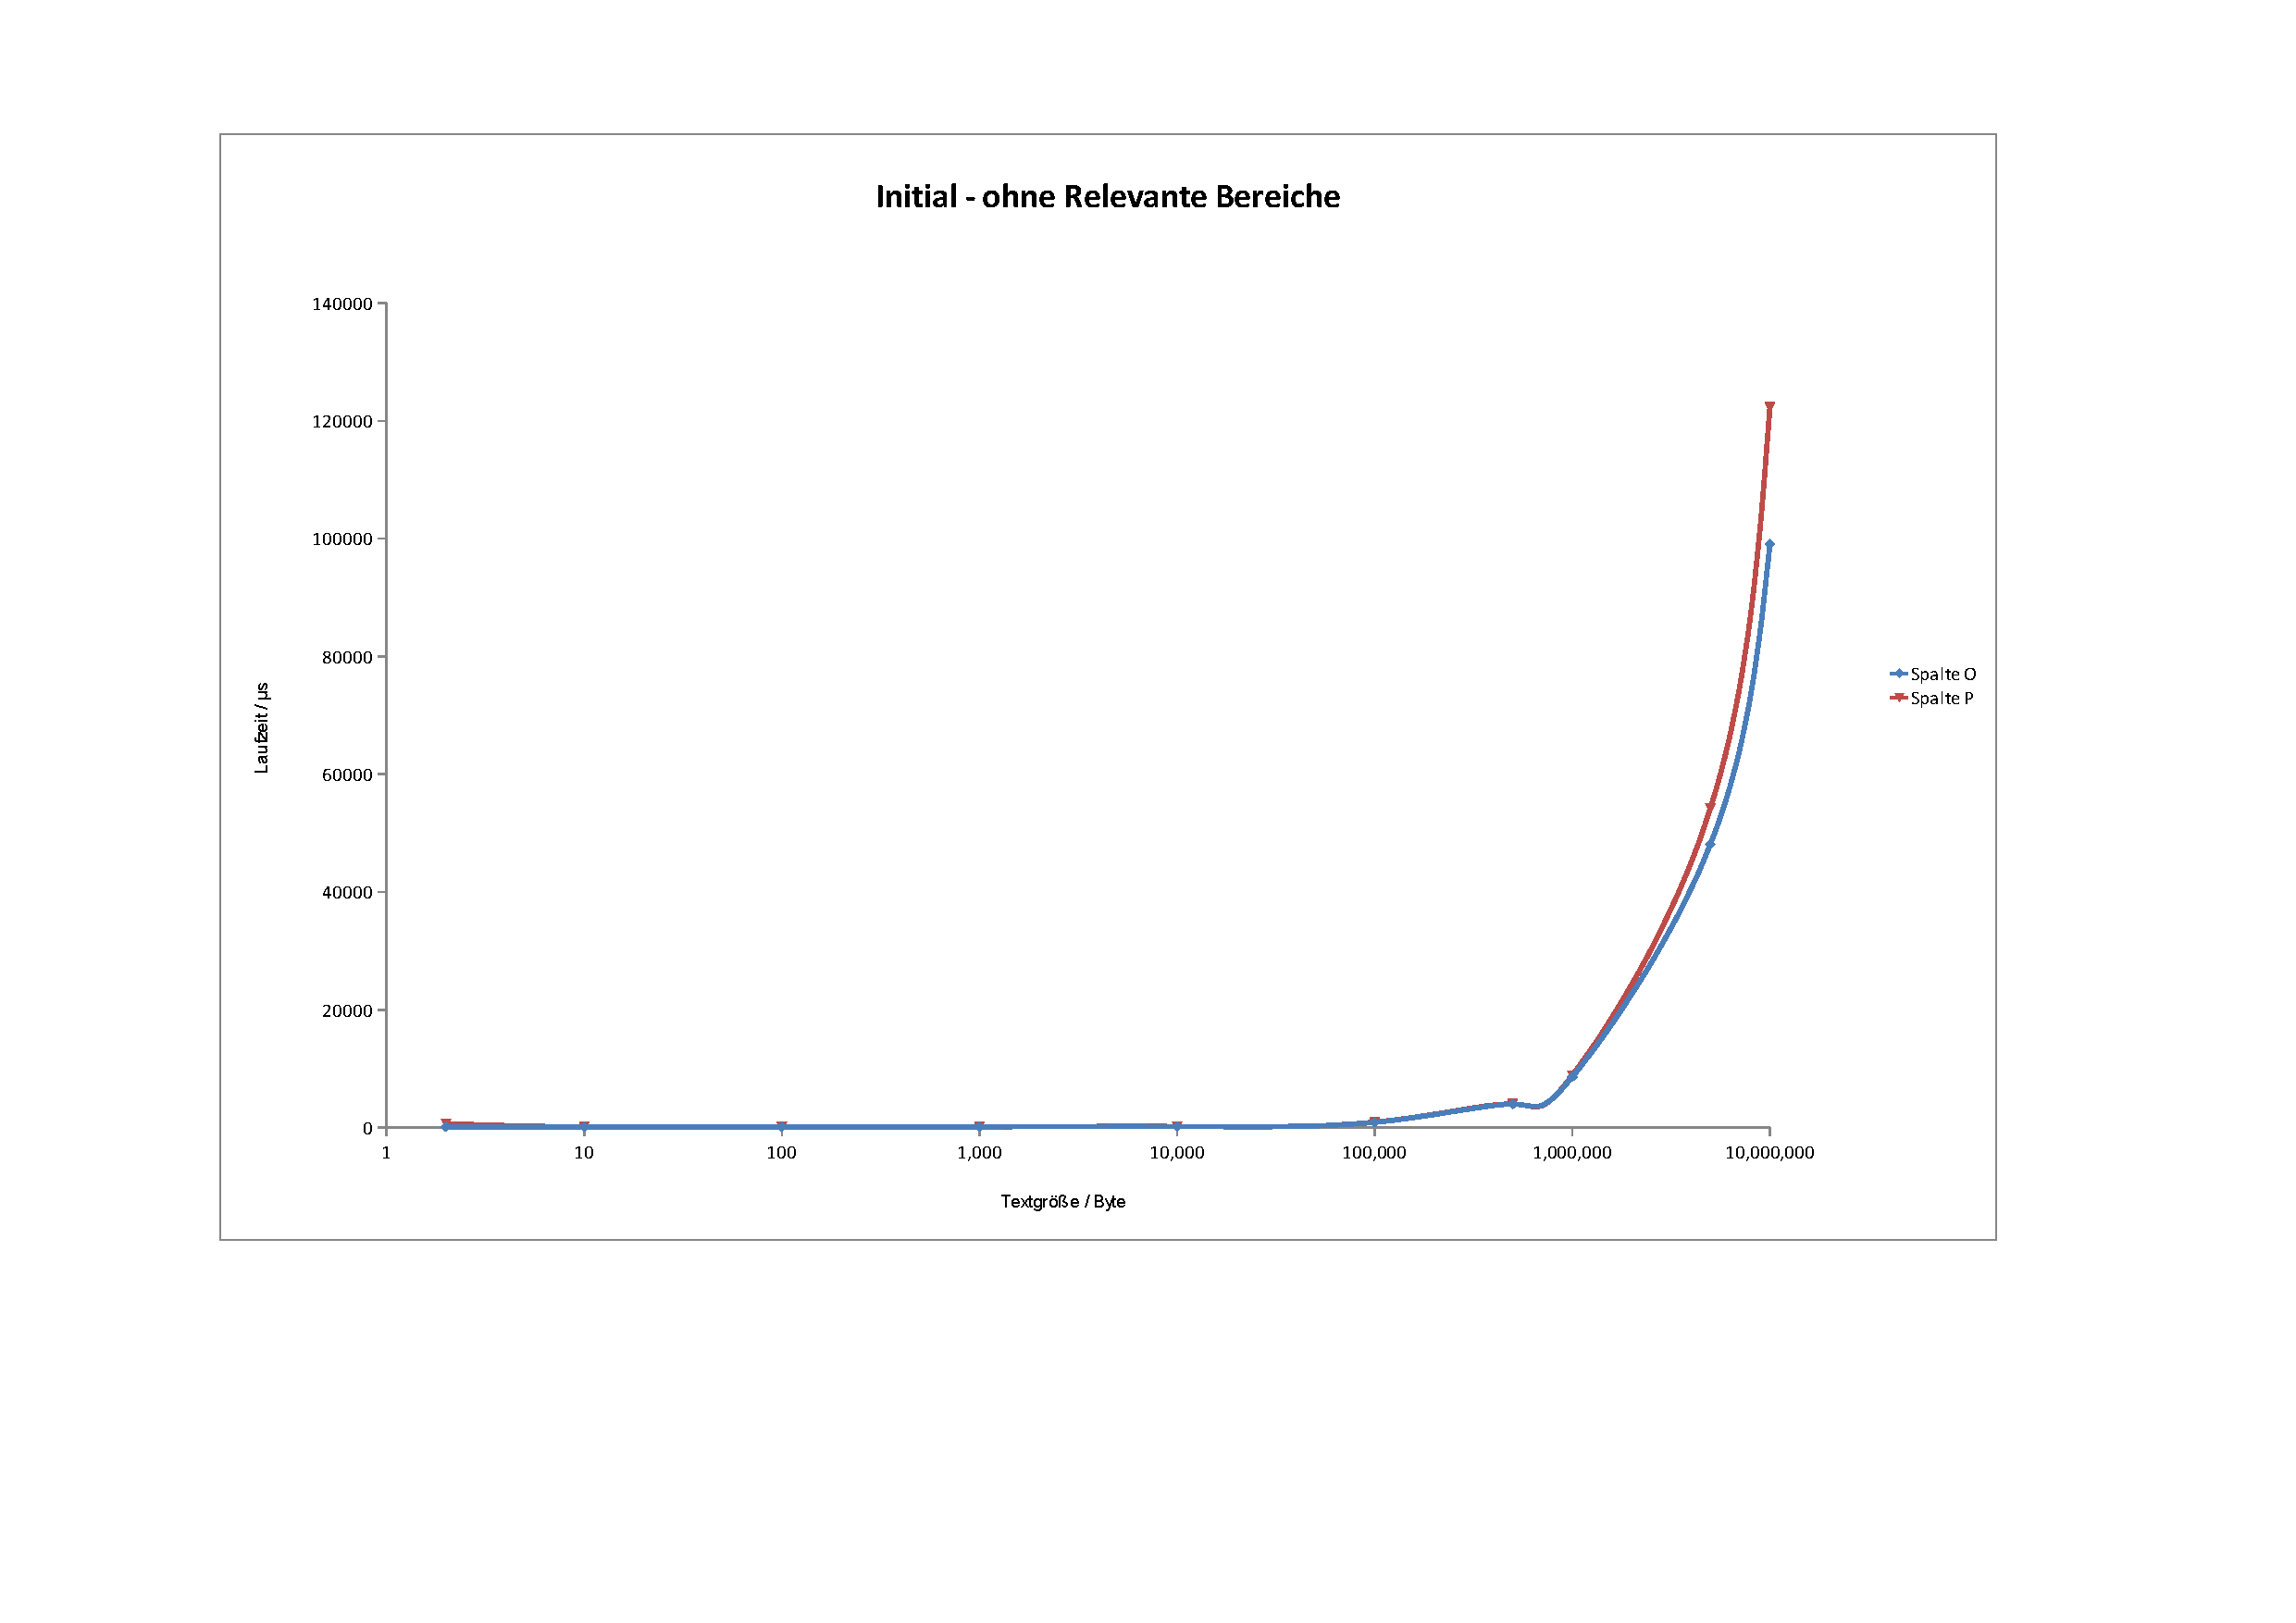
\includegraphics[scale=.45]{DiagrammInitial_worp.pdf}
	\caption{Messung-Initial ohne relevante Bereiche}
	\label{fig:diagrammInitial_worp}	
\end{figure}

Der Nachteil gegenüber der Quellcodegrößenoptimierung liegt darin, dass
mehr Speicherplatz in Anspruch genommen wird, wodurch der
Geschwindigkeitsvorteil erreicht werden kann.
Die Wahl der jeweiligen Optimierungsmöglichkeit ist situationsabhängig. Auf dem
Mars stehen weniger Speicherressourcen zur Verfügung, wodurch eine
Geschwindigkeitsoptimierung weniger sinnvoll erscheint.

%Hypothese 2
Unter der Berücksichtigung relevanter Bereiche ist eine Änderung der Laufzeit
anzunehmen. Diese sollte mit wachsender Anzahl von relevanten Bereichen
ansteigen, da zusätzliche Berechnungen anfallen, die zum Zerteilen des Textes
notwendig sind.
\newline
% Methodik 2
Zum Testen wird ein Text mit konstanter Größe von $5.000.000$ Byte
herangezogen. Dieser beinhaltet je nach Messreihe unterschiedlich viele
relevante Bereiche, von $1$ bis $1.000$. Auch hier wurde das Modul vor jeder
Messung zurückgesetzt.
% Auswertung 2
\newline
In Abbildung \ref{fig:diagrammInitial_wrp} ist die Laufzeit in
Abhängigkeit einer bestimmten Menge von wichtigen Fragementen dargestellt.
Die Textgröße bleibt dabei stetig bei $5.000.000$ Byte. Damit ist ein Vergleich mit den
durchschnittlichen Werten der gleichen Textgröße aus Abbildung
\ref{fig:diagrammInitial_worp} möglich. Für wenige relevante Bereiche
unterscheiden sich die Werte nur marginal. Steigt die Anzahl, nimmt die Laufzeit
jedoch exponentiell zu (siehe Abbildung \ref{fig:diagrammInitial_wrp}) und
bewegt sich dann im Millisekunden-Bereich. Dies bedeutet, dass die Implementierung noch
nicht für die Verwendung von einer sehr großen Anzahl optimiert wurde. Im
Kapitel \ref{sec:Anwendungsszenarien} wurden bereits mögliche
Anwendungsszenarien betrachtet, welche ebenso mit wenigen relevanten Bereichen
auskommen. Dadurch ist eine Optimierung an dieser Stelle vorerst nebensächlich.

\begin{figure}[H]
	\centering
	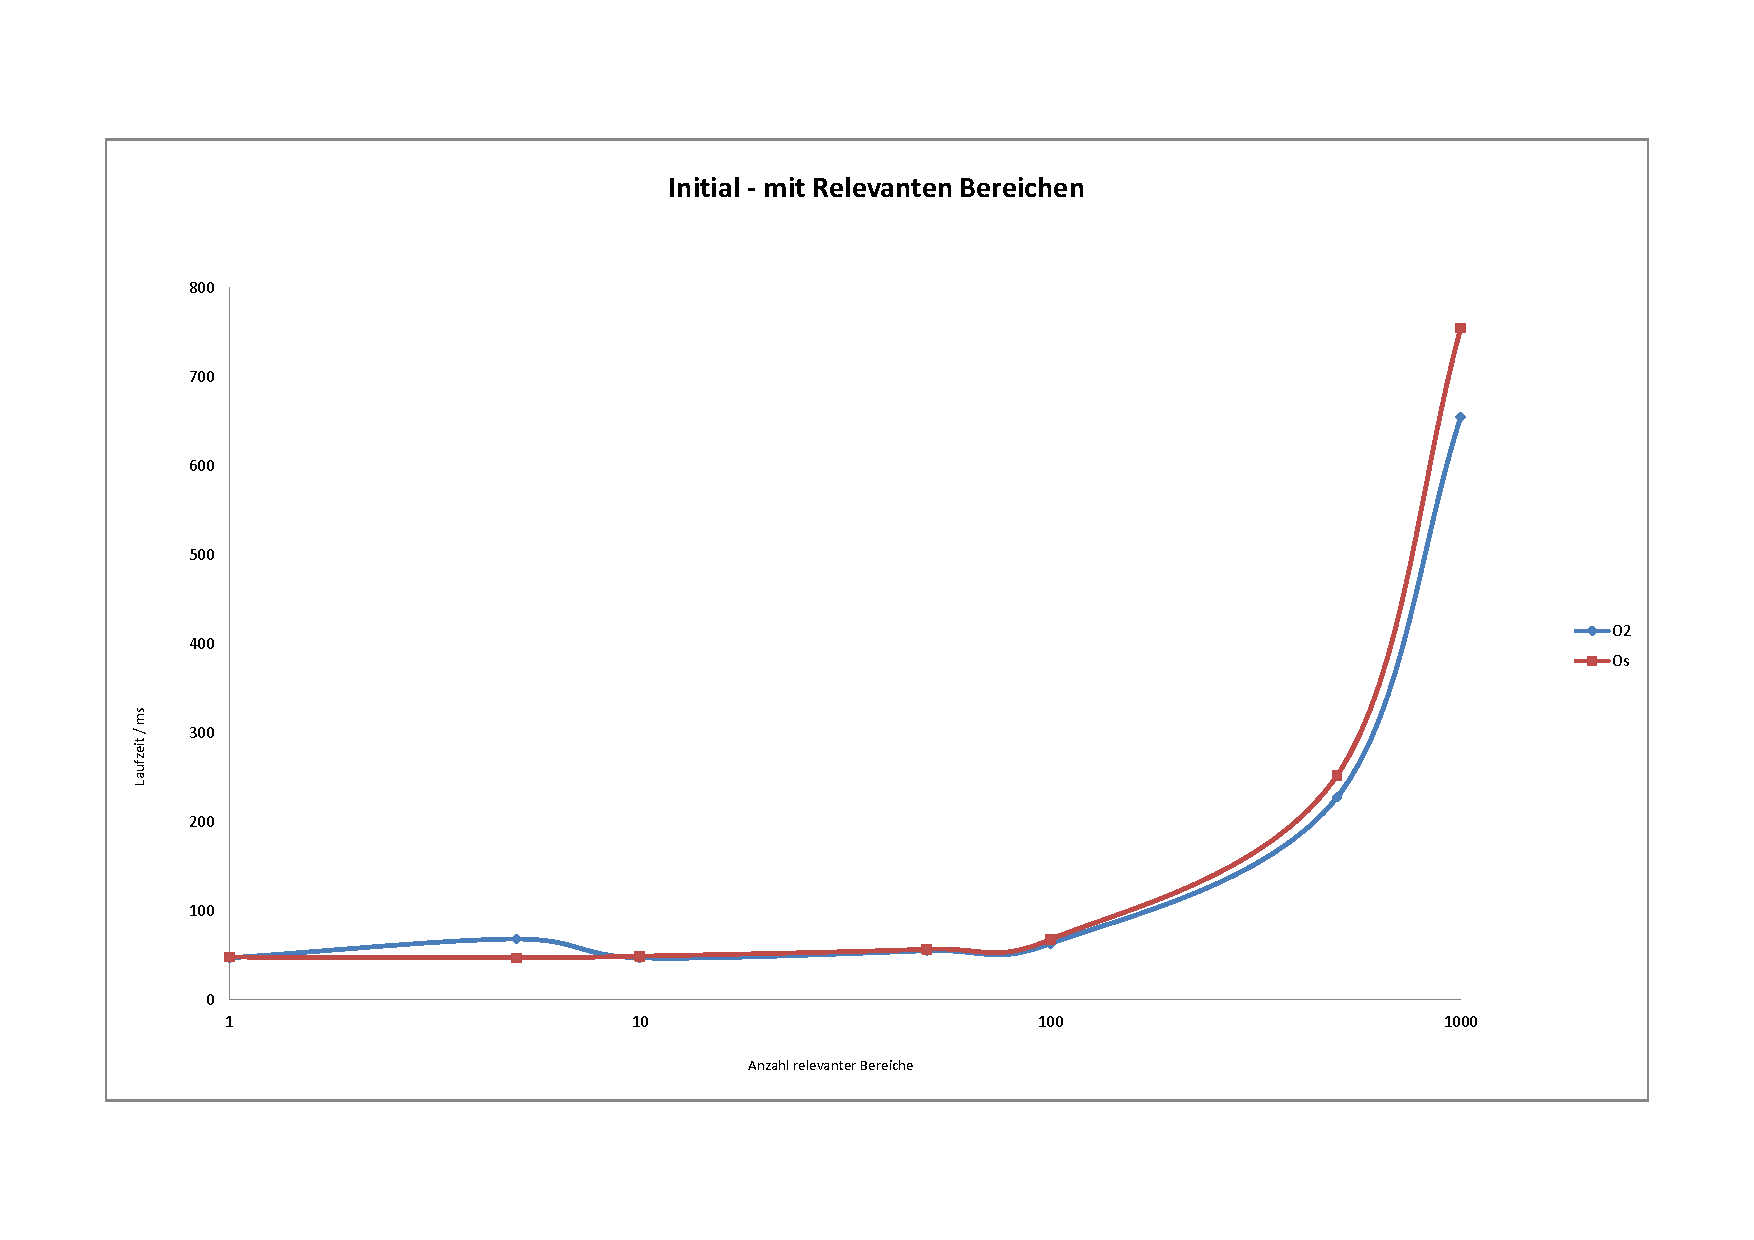
\includegraphics[width=\textwidth]{DiagrammInitial_wrp.pdf}
	\caption{Messung-Initial mit relevanten Bereichen}
	\label{fig:diagrammInitial_wrp}
\end{figure}

% Hypothese 3
Die bisherigen Untersuchungen wurden jedesmal auf Grundlage des Zurücksetzens
des Moduls betrachtet. Bei einer Messung mit durchgängig laufendem Modul sollten
sich Probleme hinsichtlich des Speicherbedarfs ergeben.
% Methodik 3
\newline
Die bisherigen Messungen werden noch einmal ohne Zurücksetzen wiederholt. Dabei
werden relevante und nicht relevante Bereiche nacheinander jeweils $10$ Mal vom
Modul verarbeitet (Verweis auf Anhang \ref{sec:messtabellen}), um den
erwarteten Effekt erzielen zu können. Damit sind insgesamt $41.400$ Datenblöcke
mit $548$ MB zu bewältigen. 
% Auswertung 3
\newline
Bei der Durchführung ist ein Anstieg der Laufzeit zu erkennen (siehe
Messwerttabelle \ref{fig:messung_normal_worp} und \ref{fig:messung_normal_wrp}),
je mehr Daten bereits verarbeitet wurden. Eine genauere Analyse zeigt, dass das
Einsortieren in die Datenstruktur \Code{SmartPrioritizedQueue} der Grund für die
Laufzeitverlängerung ist.
Dabei lagen alle Datenblöcke gleichzeitig im Speicher, wodurch das
Einsortieren neuer Blöcke sehr viel Rechenleistung in Anspruch nimmt.
Gleichzeitig werden diese Daten im Arbeitsspeicher und auf der Festplatte
hinterlegt. Hierbei gilt zu untersuchen, ob diese Form der Datensicherung bei
einem Rover auf dem Mars praktikabel ist, da dieser über sehr begrenzte
Speicherressourcen verfügt. \newline
Alternativ müssen neue Methoden gefunden werden, den
Speicherverbrauch einzuschränken. So besteht die Möglichkeit, die Daten nur auf
der Festplatte zu speichern und in der priorisierenden Datenstruktur die Indizes
zu diesen zu hinterlegen. Dadurch kann der Speicherverbrauch im Arbeitsspeicher
stark reduziert werden. Aufgrund von langen Zeiträumen in denen nicht gesendet
werden kann, wird sukzessive Speicherplatz belegt (siehe Kapitel \ref{sec:SendeZeitdauern}).
Deshalb ist diese Methode bei sehr vielen und großen Daten nicht optimal. Eine
bessere Möglichkeit wäre, anhand einer \gls{TTL} (siehe Kapitel
\ref{sec:Vorueberlegung}) unrelevante Daten nur sehr kurzfristig vorzuhalten,
damit mehr Raum für Daten von hoher Relevanz ist.
